%第五章
\chapter{标准属性}


在我们看控件之前,让我们来看看他们的一些共同指定的属性---如大小,颜色以及字体。
\begin{itemize}
\item
每个控件都有一些属性选项来影响它的显示和行为,如颜色,大小,文本标签等。
\item
当调用控件构造器时,你可以使用如text='PANIC'或者height=20等关键字参数。
\item
当你创建了一个控件后,后面你可以使用控件的.config()方法来改变参数。你也可以使用控件的.cget()方法来获取当前参数的设置。了解更多类似方法请看第26章“通用控件方法”(P.97)
\end{itemize}

%第5.1节
\section{尺寸}

控件的长,宽及其它的尺寸可以用许多不同的单位。
\begin{itemize}
\item
如果你想设置一个整数尺寸,它将默认以像素为单位
\item
你可以在设定尺寸时在数字后加入如下字符来指定单位:
\end{itemize}
\hspace{4em}
表3.尺寸单位

\hspace{2em}
\begin{tabular}{r|l}
\hline
c & Centimeters \\ \hline
i & Inches \\ \hline
m & Millimeters \\ \hline
p & Printer's points (about 1/72'') \\ \hline
\end{tabular}

\section{坐标系}
%As in most contemporary display systems, the origin of each coordinate system is at its upper left corner,
%with the x coordinate increasing toward the right, and the y coordinate increasing toward the bottom:
当前的大多数显示系统中,坐标系是在左上角,x轴向右走,y轴向下走:

\begin{figure}[H]
\hspace{1em}
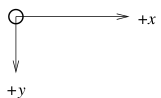
\includegraphics[width=5.680cm,height=3.457cm]{5.2.png}
\end{figure}

%The base unit is the pixel, with the top left pixel having coordinates (0,0). Coordinates that you specify
%as integers are always expressed in pixels, but any coordinate may be specified as a dimensioned
%quantity; see Section 5.1, “Dimensions” (p. 9).
最基本的单位是像素,最左上的像素的坐标为(0,0)。你所指定的整数坐标通常默认以像素为单位,但是坐标都可能指定数值;请见第5.1节“尺寸”(P.9)

%第5.3节
\section{颜色}
\textit{Tkinter}中一般有两种方法来指定颜色
\begin{itemize}
\item
你可以通过16进制字符设置红、绿、蓝颜色的比例来设置颜色:
\\
\begin{tabular}{|l|l|}
\hline
\textsf{\#rgb} & Four bits per color \\ \hline
\textsf{\#rrggbb} & Eight bits per color \\ \hline
\textsf{\#rrrgggbbb} & Twelve bits per color \\ \hline
\end{tabular}
\\
%For example, '#fff' is white, '#000000' is black, '#000fff000' is pure green, and '#00ffff'
%is pure cyan (green plus blue).
例如,“\textsf{\#fff}”是白色,“\textsf{\#000000}”是黑色,“\textsf{\#000fff000}”是纯绿色,“\textsf{\#00ffff}”是青色(绿色加蓝色)
\item
另外你也可以使用内置的标准颜色名。\textsf{white}白色,\textsf{black}黑色,\textsf{red}红色,\textsf{green}绿色,\textsf{blue}蓝色,\textsf{cyan}青色,\textsf{yellow}黄色,\textsf{magenta}品红都能用。其它颜色名也许也能用,要看本地安装环境。

\end{itemize}